\chapter{Implementering} \label{implementering}

%Her beskrives kort hvordan projektets HW-dele og SW-dele er implementeret (”lavet”). HW-delene kan med fordel beskrives med få, udvalgte, tydelige fotos. Her beskrives også kort hvordan SW-delene er implementeret (kodet). Den/de anvendte compilere beskrives meget kort (programmeringssprog, version etc.). Der argumenteres for valg af program- meringssprog. Der vises kun source code i projektrapporten, når der er tale om ekstremt interessante, små kodeudsnit. Der henvises til projektets bilag, hvor relevante/tydelige fotos af projektets HW og den samlede source code for projektets SW er anbragt.

\section*{Indledning}
Dette kapitel har til formål at beskrive, hvorledes detekteringssystemets hardwarekomponenter samt softwarefunktioner er implementeret. 

\section{Hardware}
Den fysiske installation af hardwarekomponenterne er realiseret og sammenkoblet ved simpel implementering. Dermed er det let at overskue, optimere samt fejlsøge systemet. Som beskrevet i hardware design, se afsnit \ref{hardwaredesign}, er det forsøgt at benytte hardwarekomponenter, som i forvejen anvendes klinisk. Dermed er systemet nemmere at implementere hos slutbrugeren. 

På Figur \ref{Implementering1} ses en illustration af, hvorledes de forskellige hardwarekomponenter er implementeret. 

\begin{figure}[H]
	\centering
	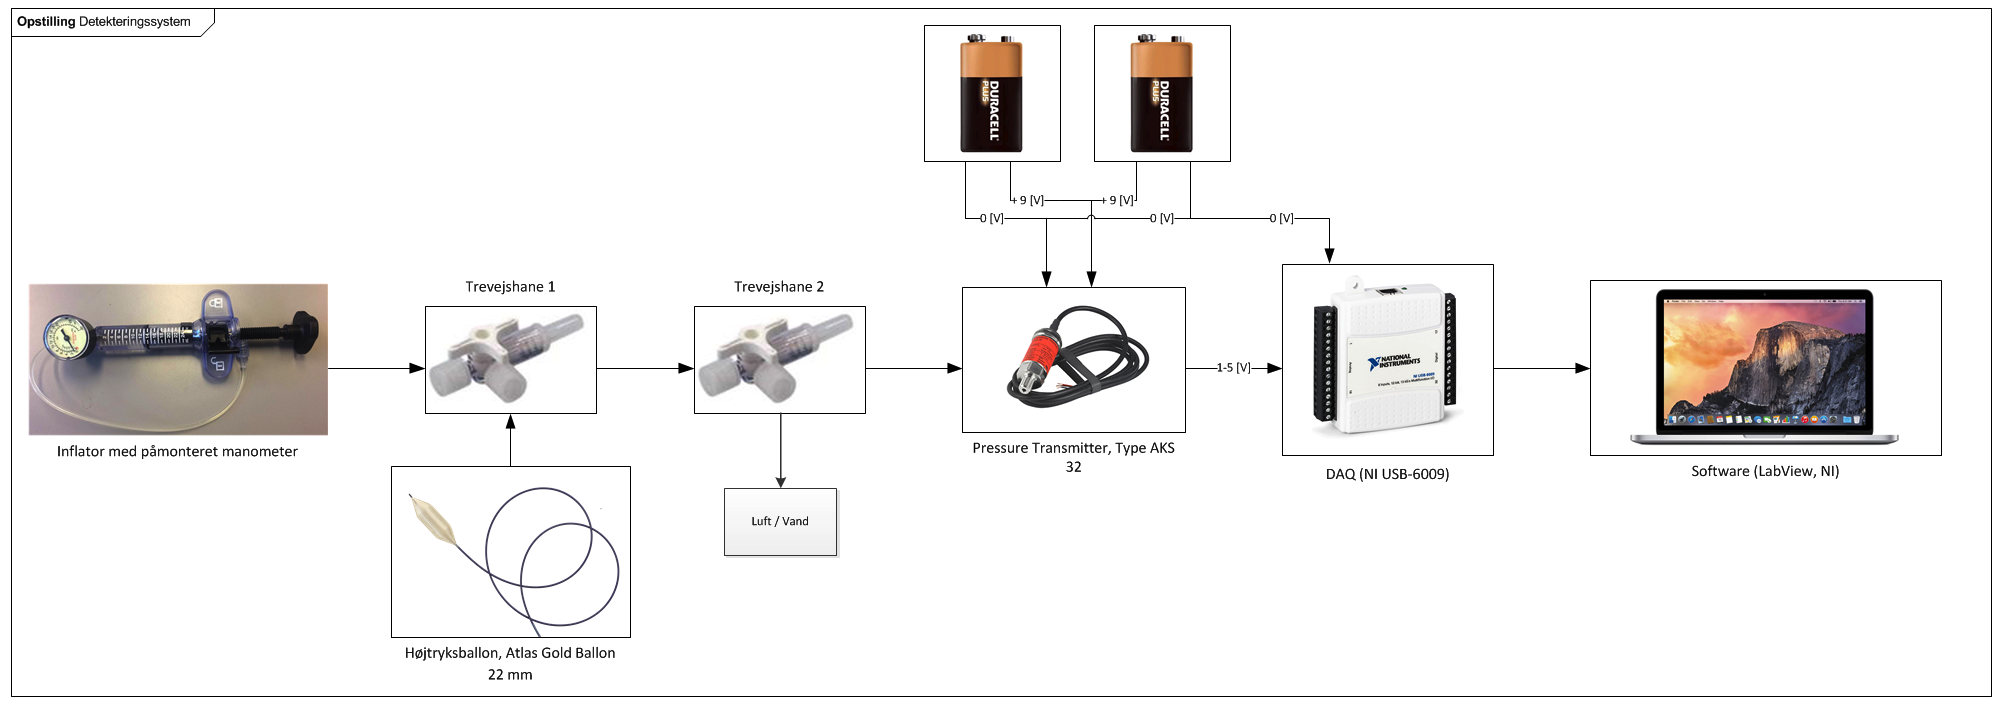
\includegraphics[width=1\textwidth]{Figure/HW_implementering}
	\caption{Illustration af hvorledes hardwarekomponenterne er implementering}
    \label{Implementering1}
\end{figure}

Inflatoren er forbundet til trevejshane 1, som endvidere er forbundet til trevejshane 2, samt til højtryksballonen. Trevejshane 2 er forbundet til tryktransduceren, som er forsynet med strøm fra to 9 volts batterier, som samlet leverer en spænding på 18 V. Tryktransduceren er videre forbundet til DAQ'en, som via en USB port er tilkoblet computeren, hvorfra softwaren kører. 

På Figur \ref{Implementering2} ses et billede, hvor hardwarekomponenterne er forbundet med hinanden og dermed implementeret. 

\begin{figure}[H]
	\centering
	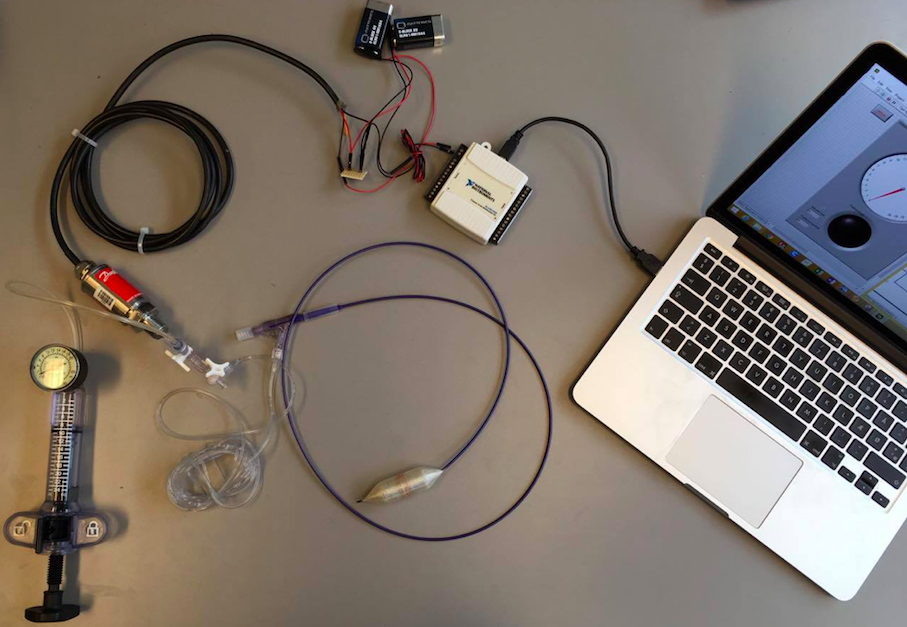
\includegraphics[width=0.7\textwidth]{Figure/Implementering}
	\caption{Implementering af hardwarekomponenter}
    \label{Implementering2}
\end{figure}

For ydeligere beskrivelse af hardware implementering, se dokumentationen afsnit 4.2.     

\section{Software}
Detekteringssystemets software er programmeret i LabVIEW. I dette afsnit vil implementeringen af de to vigtigste softwarefunktioner blive beskrevet. På Figur \ref{SW_1} ses den overordnet kodestruktur for implementeringen af detekteringssystemet. 

\begin{figure}[H]
	\centering
	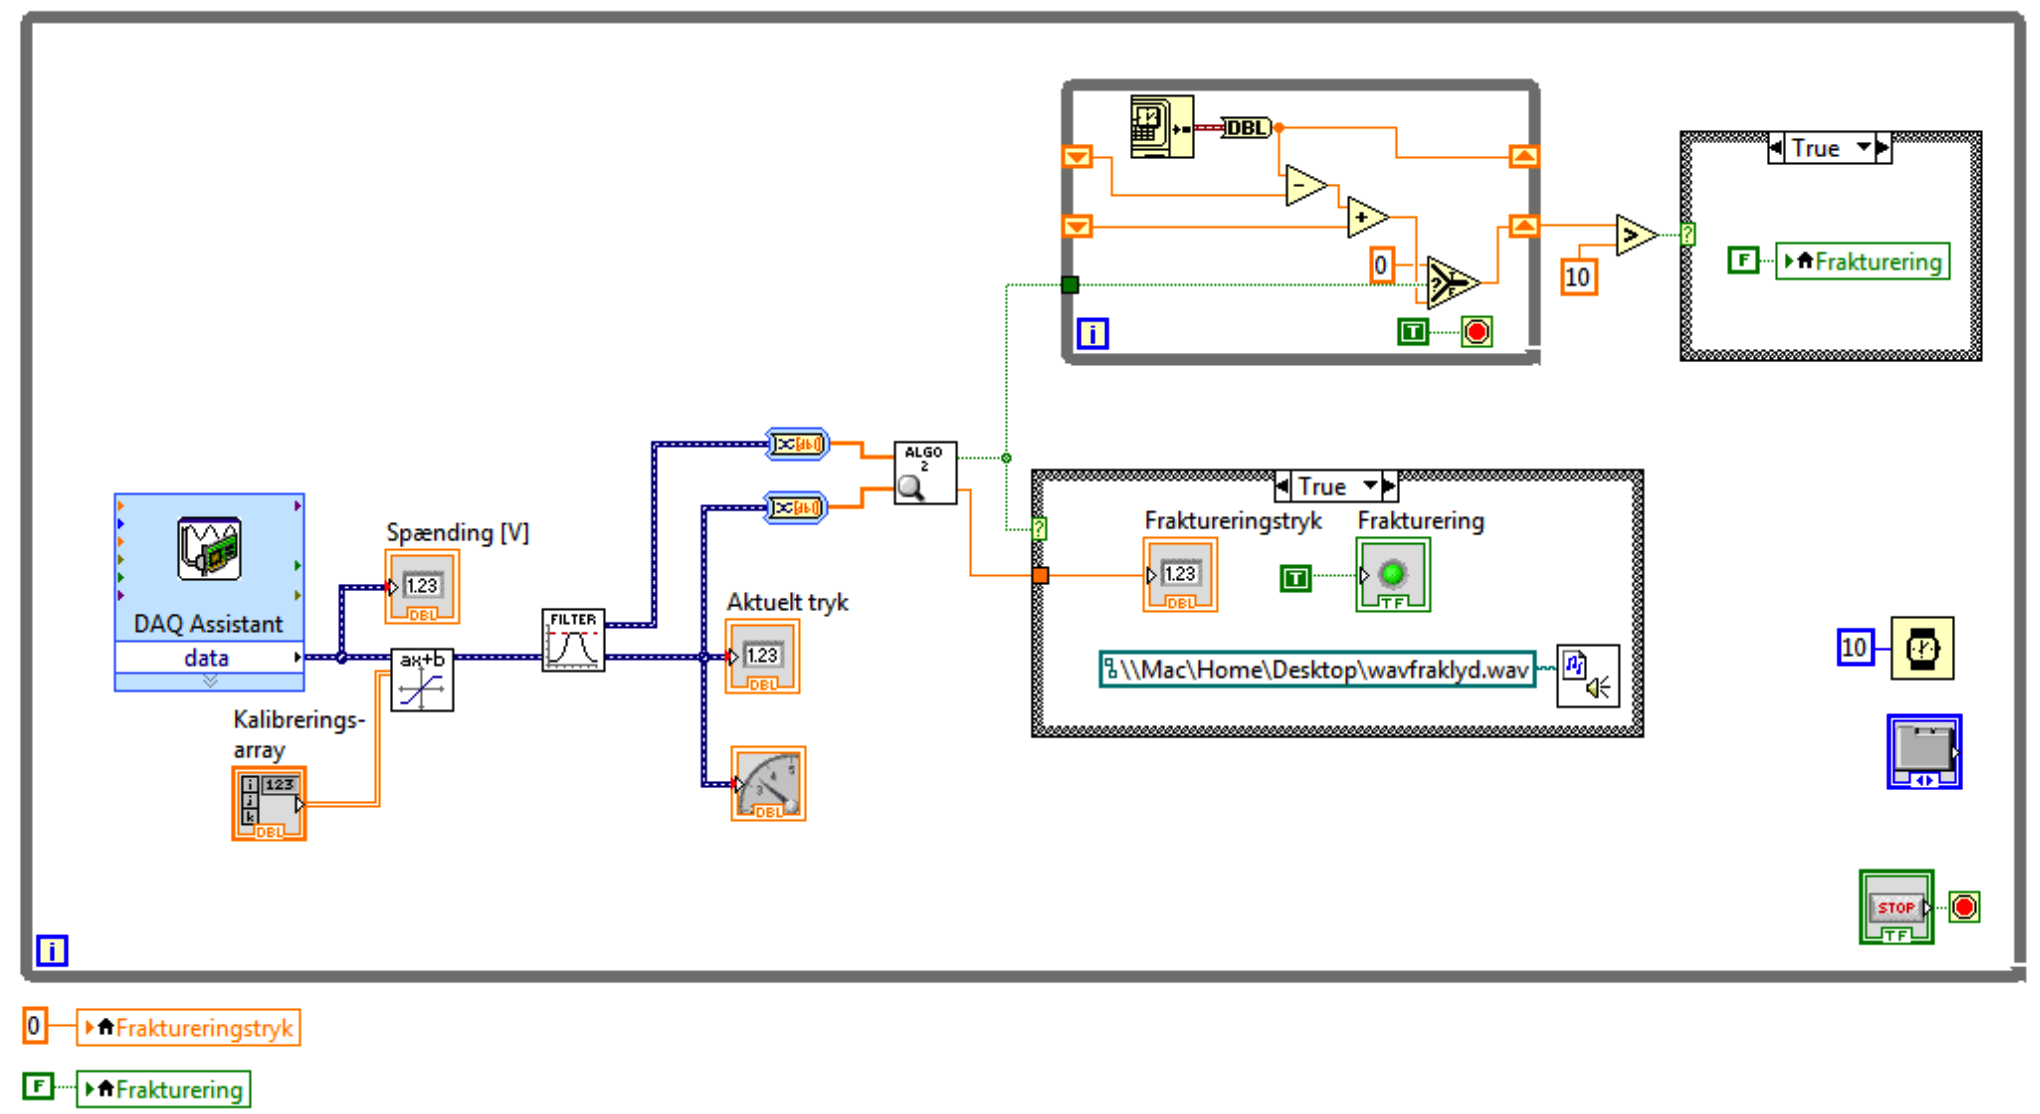
\includegraphics[width=1\textwidth]{Figure/SW_1}
	\caption{Overordnet kodestruktur for detekteringssystemet}
	\label{SW_1}
\end{figure} 

Koden består af en while-løkke (den store grå boks, som omkranser den primære del af koden). De to variabler uden for while-løkken er default værdier, der sikrer, at den numeriske indikator 'Fraktureringstryk' samt 'Frakturering'-lampen på detekterings GUI'en er henholdvis 0 og 'false' (slukket) indtil en detektering har fundet sted. 

Den vigtigste softwarefunktion er 'Detekteringsalgoritme', som sikrer, at en frakturering detekteres og informerer operatøren herom på brugergrænsefladen. Forinden 'Detekteringsalgoritme' kan fungere er det vigtigt, at signalet bliver filtret. 


\subsection{Digitale filtre}
På Figur \ref{SW_2} er koden for softwarefunktionen 'Digitale filtre' (lille rød firkant) foldet ud. Der er implementeret to filtre: et lavpas- og et højpasfiltrer, hvis design er beskrevet i afsnit \ref{SW_design_filtre} samt i dokumentationen afsnit 5.1.2. Hvorledes specifikationerne for hvert filter er blevet implementeret, står beskrevet i dokumentationen afsnit 5.2.2. 


\begin{figure}[H]
	\centering
	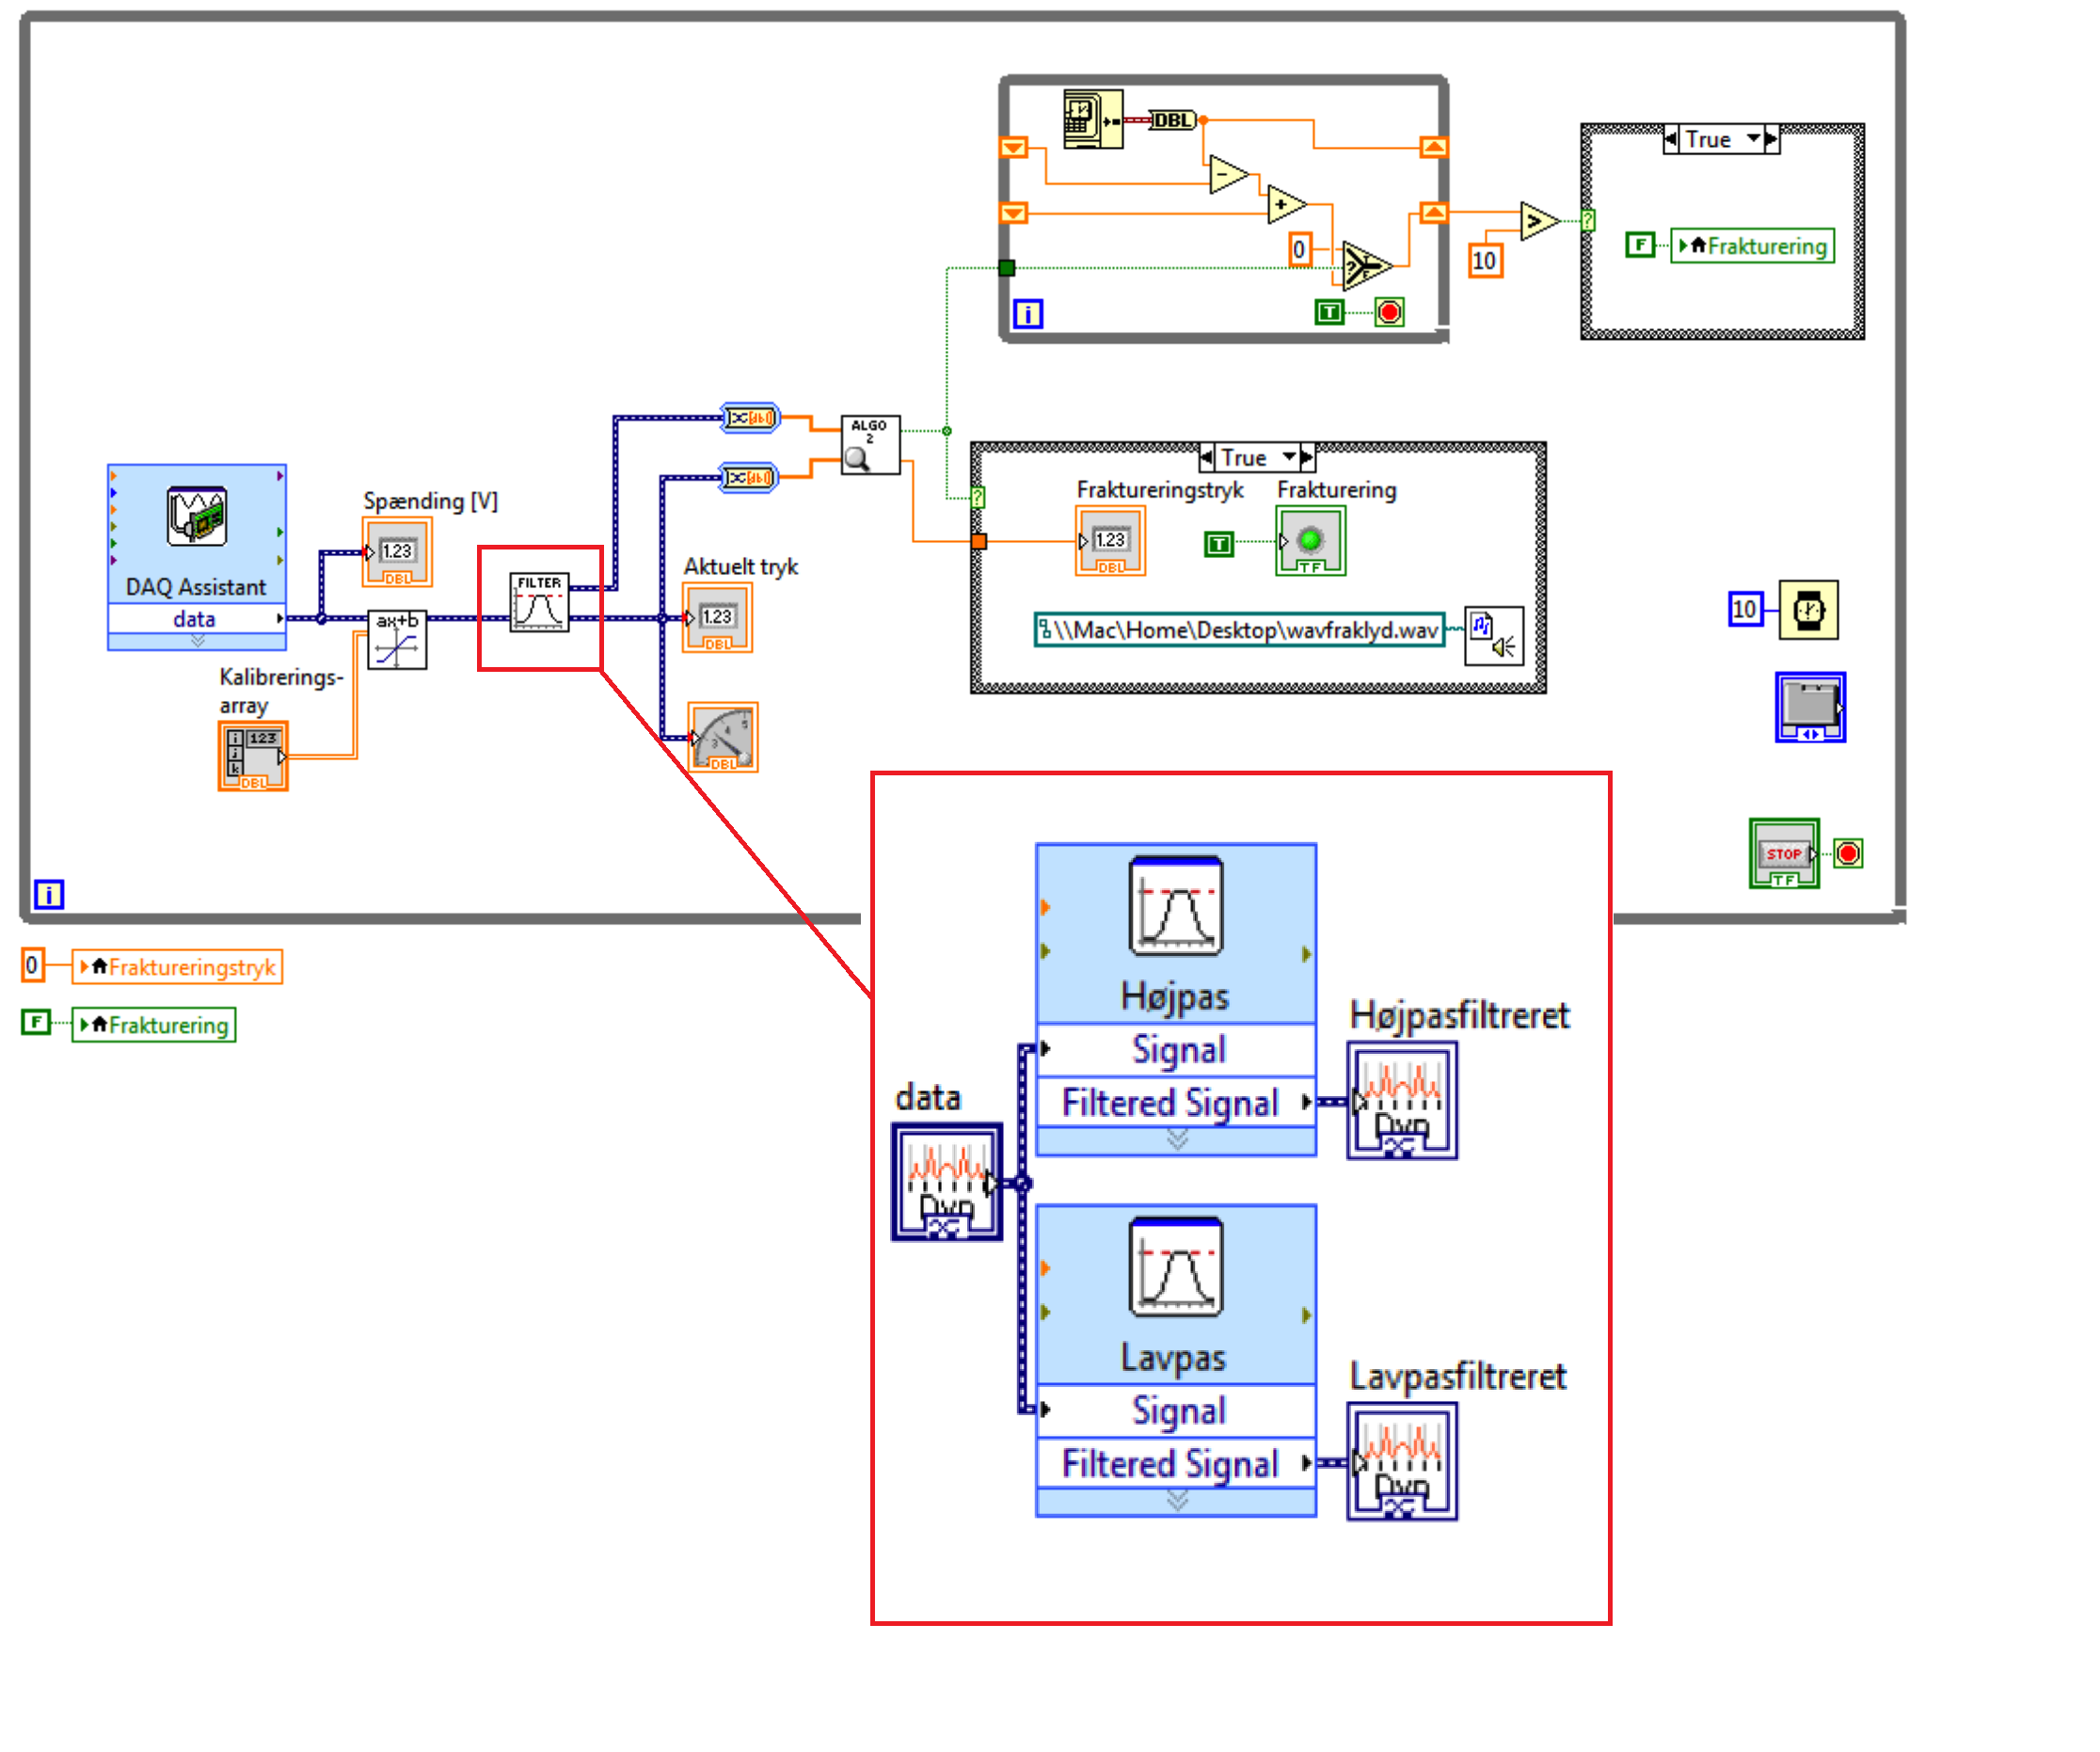
\includegraphics[width=1\textwidth]{Figure/SW_3}
	\caption{Kodestruktur for digital filtrering}
	\label{SW_2}
\end{figure} 

Signalet, som DAQ assistant har indlæst, bliver henholdsvis lavpas- og højpasfiltreret. Softwarefunktionen 'Digitale filtre' har to udgangstråde. Den ene er det lavpasfiltrerede signal, som sikrer en stabil visning af det aktuelle tryk på detekterings GUI'en, mens det højpasfiltrerede signal løber op til og skal anvendes i softwarefunktionen 'Detekteringsalgoritme'. 

\subsection{Detekteringsalgortime}
På Figur \ref{SW_4} er koden for softwarefunktionen 'Detekteringsalgoritme' (lille rød firkant) foldet ud. 

\begin{figure}[H]
	\centering
	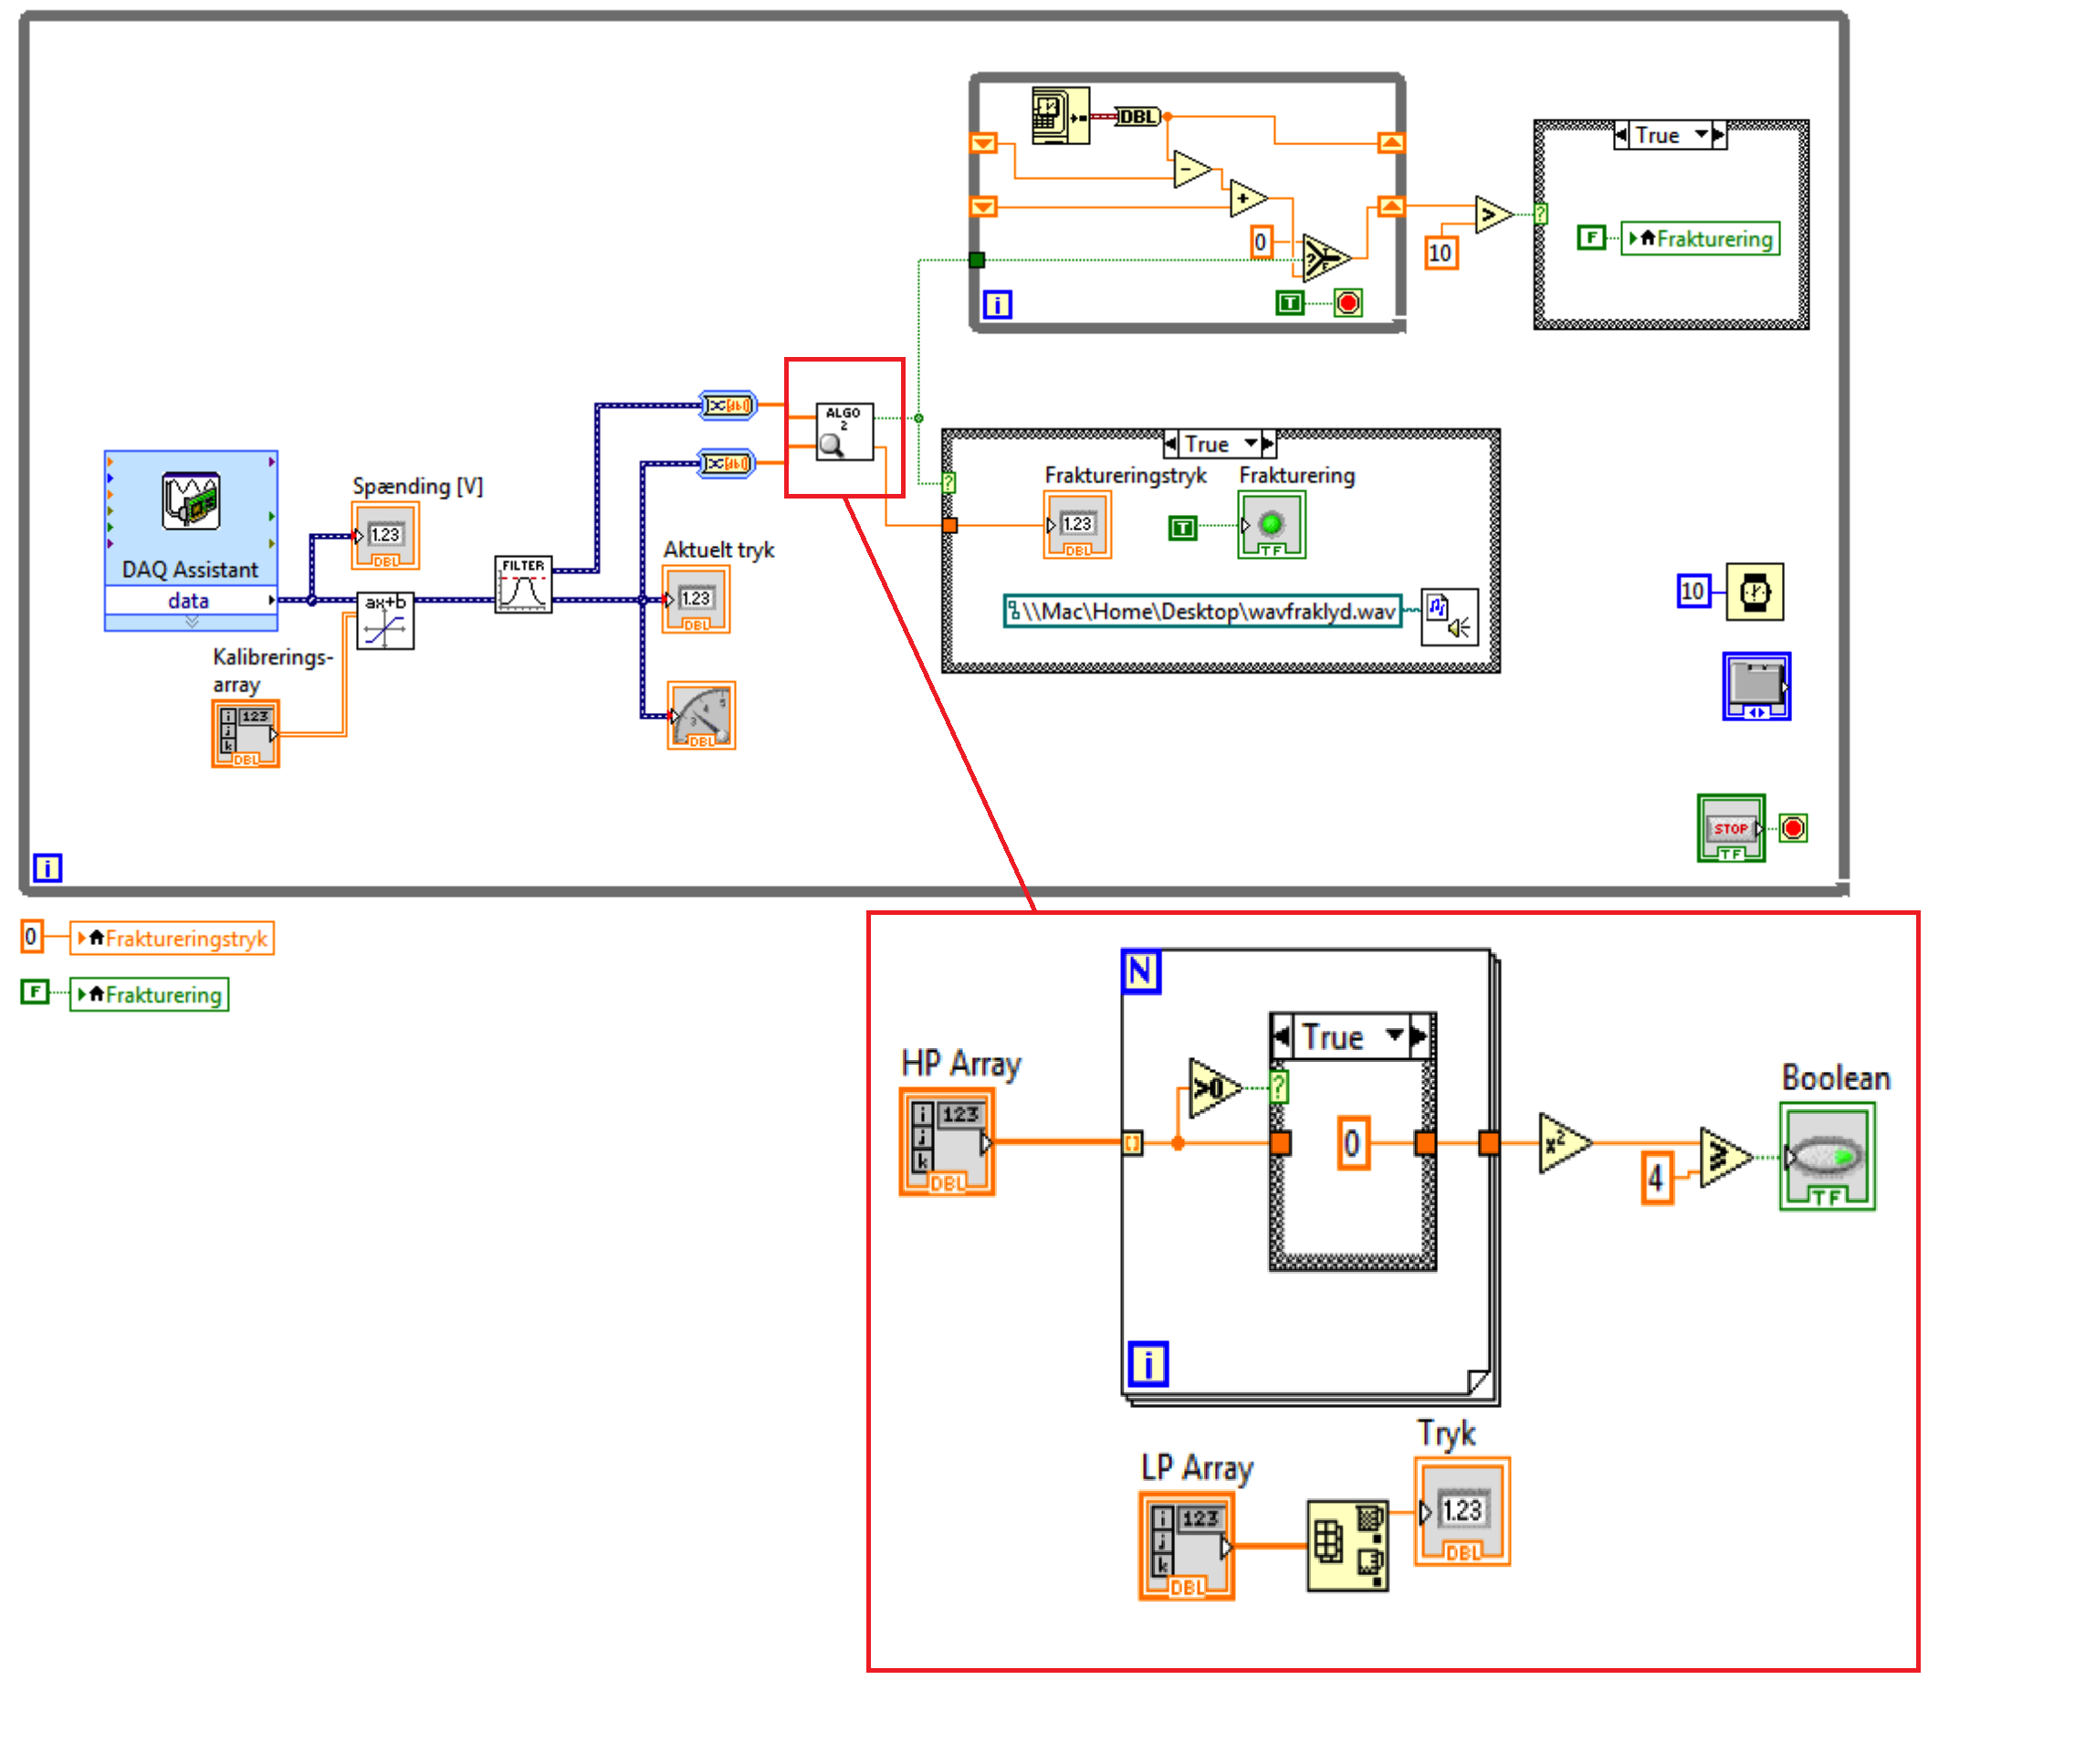
\includegraphics[width=1\textwidth]{Figure/SW_4}
	\caption{Kodestruktur for detekteringsalgoritmen}
	\label{SW_4}
\end{figure} 

Det højpasfiltrerede signal løber ind i en for-løkke og videre ind i en case-struktur, som på Figur \ref{SW_4} er sat til at være 'true'. Den tjekker det højpasfiltrerede signal for værdier $>0$, og hvis det er 'true' sættes værdien til 0. På den måde fjernes alle positive værdier fra signalet. Signalet løber nu ud af for-løkken, hvor det bliver kvadreret. Det nu positive signal løber ind i en 'Boolean', som bliver 'true', når det positive signal har en værdi på $\geq4$. 

Nedenfor case-strukturen er et lille stykke kode, som hele tiden indlæser de sidste 100 værdier af det lavpasfiltrerede signal og gemmer den højeste værdi.    

Udfra 'Detekteringsalgoritme' er der to tråde, hvor den ene løber ind i en case-struktur (den nederste), mens den anden løber ind i en while-løkke (den øverste). Når den boolske-værdi i 'Detekteringsalgoritme' er 'true', forekommer case-strukturen, som vist på Figur \ref{SW_4}. Her bliver 'Frakturering's-lampen på detekterings GUI'en tændt samt en lyd bliver afspillet. Den numeriske indikator 'Fraktureringstryk' på detekterings GUI'en ændres fra defaultværdien 0 til den højeste værdi, der er blevet gemt i 'Detekteringsalgoritme'. While-løkkens funktion er at sikre, at frakturerings-lampen bliver slukket igen efter 10 sekunder. While-løkken har hele tiden styr på tiden siden sidste 'true'. Det vil sige, når en frakturering forekommer og den boolske-værdi er 'true' nulstilles tiden i while-løkken. Når tiden overstiger 10 sekunder bliver den sidste case-struktur 'true' og 'Frakturering's-lampen bliver 'false' og slukker.    

Hvorledes de andre softwarefunktioner er blevet implementeret er beskrevet i dokumentation afsnit 5.2. Endvidere kan hele source code for detekteringssystemet ses i Bilag 15.    





